\documentclass{article}
\usepackage{amsmath}
\usepackage{graphicx}
\usepackage[colorlinks=true, linkcolor=black, citecolor=cyan, urlcolor=darkgray]{hyperref}
\usepackage{dirtree}
\usepackage{hyperref}
\usepackage{tikz}
\usetikzlibrary{automata, positioning, arrows}

\usepackage{xepersian}
\settextfont{B Nazanin}

\newcommand{\english}[1]{\settextfont{Times New Roman} \lr{#1} \settextfont{B Nazanin}}

\title{تشخیص عواطف توسط دستگاه‌های پوشیدنی}
\begin{document}
	\maketitle
	\newpage
	\begin{abstract}
		تشخیص عواطف یکی از کاربردهای روزافزون هوش مصنوعی است. این کار می‌تواند در صنعت روانشناسی و خصوصا حوزه ترکیبی محاسبات عاطفی نقش بسیار پررنگی ایفا کند. همچنین هر روز پیشرفت بیشتری را در مورد پوشیدنی‌های هوشمند و افزایش استفاده از آنها را شاهد هستیم.
	\end{abstract}
	\newpage
	\tableofcontents
	
	\section{عواطف}
	
	\section{مجموعه داده}
	مجموعه داده \english{WESAD\cite{wesad}} یکی از کامل‌ترین ﻣﺠﻤﻮﻋﻪ ﻫﺎﻱ ﺩﺍﺩﻩ ﺑﺮﺍﻱ ﺗﺸﺨﻴﺺ ﻋﻮﺍﻃﻒ ﺍﺳﺖ. ﺑﻴﺸﺘﺮﻳﻦ ﺗﻤﺮﻛﺰ ﻭ ﺍﺳﺘﻔﺎﺩﻩ ﺍﺯ ﺍﻳﻦ ﻣﺠﻤﻮﻋﻪ ﺑﺮﺍﻱ ﺗﺸﺨﻴﺺ ﺍﺳﺘﺮﺱ ﺑﻮﺩﻩﺍﺳﺖ. ﺑﺎ ﺍﻳﻦ ﻭﺟﻮﺩ، ﺑﻪ ﺟﺰ ﻛﻼﺱ ﺍﺳﺘﺮﺱ ﻭ ﻋﺎﺩﻱ، ﺑﺮﺍﻱ ﻧﺸﺨﻴﺺ ﻛﻼﺱ ﻫﺎﻱ ﺧﻮﺷﺤﺎﻟﻲ ﻭ ﺁﺭﺍﻣﺶ ﻧﻴﺰ ﻣﻲﺗﻮﺍﻥ ﺍﺯ ﺍﻳﻦ ﺩﺍﺩﻩﻫﺎ ﺍﺳﺘﻔﺎﺩﻩ ﻧﻤﻮﺩ. ﻋﻼﻭﻩ ﺑﺮ ﺁﻥﻫﺎ، ﻫﺮ ﺷﺨﺺ پﺮﺳﺸﻨﺎﻣﻪﻫﺎﻳﻲ ﻧﻴﺰ پﺮ ﻛﺮﺩﻩ ﻛﻪ ﺍﻳﻦ ﻫﻢ ﻣﻲﺗﻮﺍﻧﺪ ﺑﺎﻋﺚ ﺧﻠﻖ ﻣﺪﻝ ﻫﺎﻱ ﺟﺪﻳﺪﻱ ﺷﻮﺩ. ﺩﻭ ﺩﺳﺘگﺎﻩ ﺍﺻﻠﻲ ﺑﺮﺍﻱ ﻓﺮﺍﻫﻢ ﺁﻭﺭﺩﻥ ﺍﻳﻦ ﺩﺍﺩﻩﻫﺎ ﻣﻮﺭﺩ ﺍﺳﺘﻔﺎﺩﻩ ﻗﺮﺍﺭ گﺮﻓﺘﻪ ﺍﻧﺪ: \textbf{1(} مچ‌بند \english{Emaptica E4} ﻪ ﺑﺴﻴﺎﺭﻱ ﺍﺯ ﺩﺍﻧﺸگﺎﻩﻫﺎﻱ ﺳﺮﺍﺳﺮ ﺩﻧﻴﺎ ﺍﺯ ﺁﻥ ﺍﺳﺘﻔﺎﺩﻩ ﻣﻲ ﻛﻨﻨﺪ\cite{empatica} و  \textbf{2(} دستگاه \english{Repiban} که یکی از پیشرفته ترین سنسورهای تحقیقاتی است که بر روی سینه نصب می‌شود\cite{respiban}.
	
	\begin{figure}
		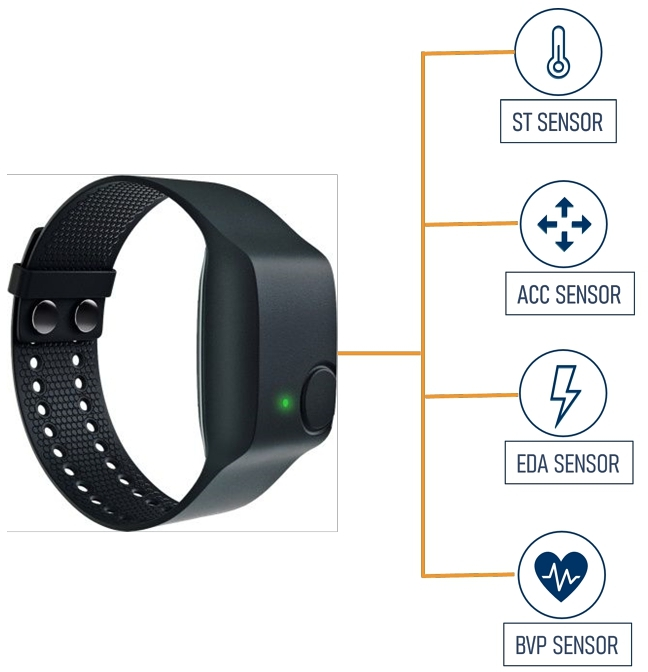
\includegraphics[width=0.5\textwidth]{empatica.jpg}
		\hspace{1cm}
		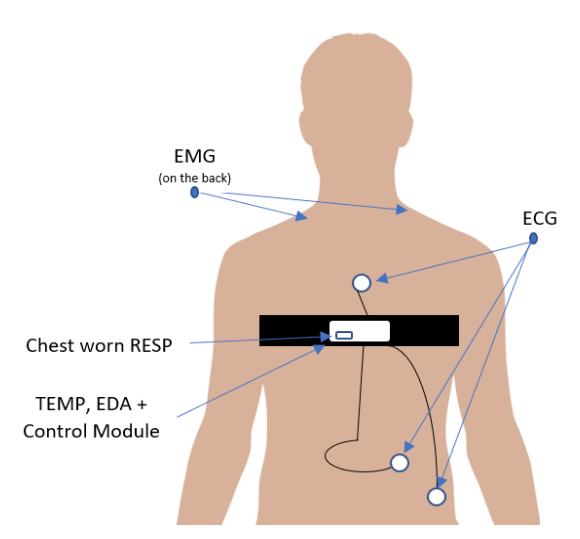
\includegraphics[width=0.5\textwidth]{respiban.png}
		\caption{شکل راست: ساعت \english{Empatica E4} ﺭﺍ ﻧﺸﺎﻥ ﻣﻲﺩﻫﺪ. ﺍﻳﻦ ﺳﺎﻋﺖ ﺑﻪ ﺩﻟﻴﻞ ﺳﻨﺴﻮﺭﻫﺎﻱ ﻛﺎﻣﻞ، ﺯﻳﺒﺎﻳﻲ ﻭ ﺭﺍﺣﺘﻲ ﺍﺳﺘﻔﺎﺩﻩ ﻛﺎﺭﺑﺮﺩ ﺯﻳﺎﺩﻱ ﺩﺭ ﺗﺤﻘﻴﻘﺎﺕ ﺩﺍﺭﺩ. 
		شکل چپ:‌ دستگاه \english{Respiban} ﻭ ﻧﺤﻮﻩ ﻗﺮﺍﺭگﻴﺮﻱ ﺁﻥ ﺭﻭﻱ ﺳﻴﻨﻪ ﻭ ﻣﺤﻞ ﻫﺮ ﻳﻚ ﺍﺯ ﺳﻨﺴﻮﺭﻫﺎ ﺭﺍ ﻧﺸﺎﻥ ﻣﻲ ﺩﻫﺪ.}
	\end{figure}
	\subsection{دستگاه \english{Respiban}}
	ﺍﻳﻦ ﺩﺳﺘگﺎﻩ ﻣﻲﺗﻮﺍﻧﺪ ۶ ﻋﺎﻣﻞ ﺭﺍ ﺍﻧﺪﺍﺯﻩگﻴﺮﻱ ﻛﻨﺪ. ﻓﺮﻛﺎﻧﺲ ﻭﺭﻭﺩﻱ ﺍﻳﻦ ﺩﺳﺘگﺎﻩ ﺑﺮﺍﻱ ﻫﻤﻪ ﺳﻨﺴﻮﺭﻫﺎﻳﺶ ۷۰۰ ﻫﺮﺗﺰ ﻣﻲﺑﺎﺷﺪ. ﺳﻨﺴﻮﺭﻫﺎﻱ ﺁﻥ ﺑﻪ ﺷﺮﺡ ﺯﻳﺮ ﺍﺳﺖ:
	\begin{enumerate}
		\item مختصات‌یابی (\english{Accelerometer})
		\item نوار قلب (\english{Electrocardiogram})
		\item فعالیت الکتریکی پوست (\english{Electrodermal Activity})
		\item برق‌ماهیچه‌نگار (\english{Electromyogram})
		\item تنفس (\english{Respiration})
		\item دما (\english{Temperature})
	\end{enumerate}
	
	\subsection{ساعت \english{Empatica E4}}
	ﺍﻳﻦ ﺳﺎﻋﺖ ﺷﺎﻣﻞ ﺳﻨﺴﻮﺭ ﻫﺎﻱ ﻣﺨﺘﺼﺎﺕ ﻳﺎﺑﻲ، فشار خون\footnote{\english{Blood Volume Pressure}}، دما . فعالیت الکتریکی پوست است. هر یک از این ﺳﻨﺴﻮﺭﻫﺎ ﺑﺎ ﻓﺮﻛﺎﻧﺲ ﻣﺘﻔﺎﻭﺗﻲ ﺍﻧﺪﺍﺯﻩگﻴﺮﻱ ﺷﺪﻩﺍﻧﺪ. ﺩﺭ ﺟﺪﻭﻝ ﻣﻘﺪﺍﺭ ﻓﺮﻛﺎﻧﺲ ﻫﺮ ﻳﻚ ﺍﺯ ﺳﻨﺴﻮﺭﻫﺎ ﺁﻭﺭﺩﻩ ﺷﺪﻩ ﺍﺳﺖ.
	
	\begin{table}[h]
		\begin{tabular}{|c|c|}
			\hline
			سنسور & فرکانس \\
			\hline
			\english{ACC} & 32\\
			\english{BVP} & 64\\
			\english{EDA} & 4\\
			\english{Temp} & 4\\
			\hline
		\end{tabular}
	\end{table}
	\subsection{پرسشنامه‌ها}
	ﻋﻼﻭﻩ ﺑﺮ ﺩﻭ ﺩﺳﺘگﺎﻩ گﻔﺘﻪ ﺷﺪﻩ، ﻫﺮ ﻳﻚ ﺍﺯ ﺳﻮژﻩﻫﺎﻱ ﺁﺯﻣﺎﻳﺶ، پﺮﺳﺸﻨﺎﻣﻪ ﻫﺎﻳﻲ ﺭﺍ پﺮ ﻛﺮﺩﻧﺪ. ﺍﻳﻦ پﺮﺳﺸﻨﺎﻣﻪﻫﺎ ﺩﺭ ﺟﻬﺖ ﺩﺭﻳﺎﻓﺖ ﺍﻃﻼﻋﺎﺕ ﺑﻴﺸﺘﺮ ﺩﺭ ﻣﻮﺭﺩ ﺍﺣﺴﺎﺳﺎﺕ ﺍﺷﺨﺎﺹ ﺑﻪ ﻛﺎﺭ گﺮﻓﺘﻪ ﺷﺪﻧﺪ، ﺍگﺮچﻪ ﺩﺭ ﻫﻴچﻳﻚ ﺍﺯ ﻣﻘﺎﻻﺕ ﺑﺮﺭﺳﻲ ﺷﺪﻩ،ﻣﺤﻘﻘﺎﻥ ﺍﺯ ﺍﻳﻦ پﺮﺳﺸﻨﺎﻣﻪ ﻫﺎ ﺍﺳﺘﻔﺎﺩﻩ ﺍﻱ ﻧﻜﺮﺩﻧﺪ. ﺩﺭ ﻗﺴﻤﺖﻫﺎﻱ پﻴﺶﺭﻭ ﺍﻳﻦ پﺮﺳﺸﻨﺎﻣﻪﻫﺎ ﺭﺍ ﺑﺮﺭﺳﻲ ﻣﻲ ﻛﻨﻴﻢ:
	
	\subsubsection*{\english{PANAS}}
	ﺳﻮژﻩ ﻣﻲﺑﺎﻳﺴﺖ ﺑﻪ ۲۶ ﺣﺲ ﺩﺭ پﺮﺳﺸﻨﺎﻣﻪ، ﺍﺯ ۱ ﺗﺎ ۵ ﺍﻣﺘﻴﺎﺯ ﺩﻫﺪ. ﺍﻳﻦ ﺍﺣﺴﺎﺳﺎﺕ ﻋﺒﺎﺭﺗﻨﺪ ﺍﺯ: ﻓﻌﺎﻝ، پﺮﻳﺸﺎﻧﻲ، ﻋﻼﻗﻪ ﻣﻨﺪ، ﺍﻟﻬﺎﻡﺷﺪﻩ، ﺭﻧﺠﻴﺪﻩ، گﻨﺎﻫﻜﺎﺭ، ﺗﺮﺳﻴﺪﻩ، ﺩﺷﻤﻨﻲ، ﻫﻴﺠﺎﻥﺯﺩﻩ، ﻣﻐﺮﻭﺭ، ﻛﺞﺧﻠﻖ، ﻣﺸﺘﺎﻕ، ﺷﺮﻣﻨﺪﻩ، ﻫﻮﺷﻴﺎﺭ، ﻧگﺮﺍﻥ، ﻣﺼﻤﻢ، ﻣﺘﻮﺟﻪ، ﻋﺼﺒﻲ، ﻭﺣﺸﺖﺯﺩﻩ، ﺍﺳﺘﺮﺳﻲ، ﺧﺴﺘﻪ، ﺧﻮﺷﺤﺎﻝ، ﻋﺼﺒﺎﻧﻲ، ﺁﺯﺭﺩﻩﺷﺪﻥ ﻭ ﻧﺎﺭﺍﺣﺖ.
	\subsubsection*{\english{STAI}}
	ﺩﺭ ﺍﻳﻦ پﺮﺳﺸﻨﺎﻣﻪ، ﺳﻮژﻩ ﺑﻪ ﻫﺮ ﻳﻚ ﺍﺯ ﺳﻮﺍﻝ ﻫﺎﻱ ﺯﻳﺮ ﺍﺯ ۱ ﺗﺎ ۴ ﻧﻤﺮﻩ ﻣﻲ ﺩﻫﺪ:
	\begin{enumerate}
		\item ﻣﻦ ﺍﺣﺴﺎﺱ ﺭﺍﺣﺘﻲ ﻣﻲ ﻛﻨﻢ
		\item ﻣﻦ ﺍﺣﺴﺎﺱ ﻧگﺮﺍﻧﻲ ﻣﻲ ﻛﻨﻢ
		\item ﻣﻦ ﻋﺼﺒﻲ ﻫﺴﺘﻢ
		\item ﻣﻦ ﺭﻳﻠﻜﺲ ﻫﺴﺘﻢ
		\item ﻣﻦ ﺍﺣﺴﺎﺱ ﺩﻟﻮﺍپﺴﻲ ﻣﻲ ﻛﻨﻢ
		\item ﻣﻦ ﺍﺣﺴﺎﺱ ﺭﺿﺎﻳﺖ ﻣﻲ ﻛﻨﻢ
	\end{enumerate}
	\subsubsection*{\english{SAM}}
	ﺍﻳﻦ ﺗﺴﺖ ﺷﺪﺕ ﻭ ﺧﻮﺏ ﻳﺎ ﺑﺪ ﺑﻮﺩﻥ ﺍﺣﺴﺎﺳﺎﺕ ﺭﺍ ﻣﻲ ﺳﻨﺠﺪ. ﺷﺨﺺ ﺩﻭ ﺳﻮﺍﻝ ﺭﺍ ﺩﺭ ﻣﻘﻴﺎﺱ ۱ ﺗﺎ ۹ پﺎﺳﺦ ﻣﻲ ﺩﻫﺪ: \textbf{1(} ﺣﺲ ﻣﻦ چقدر ﺧﻮﺏ ﺍﺳﺖ ﻭ \textbf{2(} ﺷﺪﺕ ﺍﻳﻦ ﺣﺲ چقدر ﺍﺳﺖ.
	\subsubsection*{\english{SSSQ}}
	ﺍﻳﻦ ﺗﺴﺖ ﻛﻪ ﻛﻮﺗﺎﻩﺷﺪﻩ ﺗﺴﺖ ﺍﺳﺘﺎﻧﺪﺍﺭﺩ \english{SSSQ} ﺍﺳﺖ، ﺩﺭ ﺯﻣﺎﻥﻫﺎﻱ ﺍﺳﺘﺮﺱ ﺍﺯ ﺷﺮﻛﺖ ﻛﻨﻨﺪگﺎﻥ گﺮﻓﺘﻪ ﺷﺪﻩ ﺍﺳﺖ. پﺮﺳﺶﺷﻮﻧﺪگﺎﻥ ﺑﻪ ﺳﻮﺍﻝﻫﺎﻱ ﺯﻳﺮ ﺍﺯ ۱ ﺗﺎ ۵ ﻧﻤﺮﻩ ﻣﻲ ﺩﻫﻨﺪ:
	\begin{enumerate}
		\item ﻣﻦ ﻣﺘﻌﻬﺪ ﺑﻪ ﺭﺳﻴﺪﻥ ﺑﻪ ﺍﻫﺪﺍﻑ ﻋﻤﻠﻜﺮﺩﻱﺍﻡ ﻫﺴﺘﻢ
		\item ﻣﻦ ﻣﻲﺧﻮﺍﻫﻢ ﺩﺭ ﺍﻳﻦ ﻛﺎﺭ ﻣﻮﻓﻖ ﺷﻮﻡ
		\item ﻣﻦ ﺍﻧگﻴﺰﻩ ﺑﺮﺍﻱ ﺍﻧچﺎﻡ ﺍﻳﻦ ﻛﺎﺭ ﺭﺍ ﺩﺍﺭﻡ
		\item ﻣﻦ ﺧﻮﺩﻡ ﺭﺍ ﺑﺮﻭﺯ ﻣﻲ ﺩﻫﻢ
		\item ﻣﻦ ﻧگﺮﺍﻥ ﺗﻔﻜﺮﺍﺕ ﺩﻳگﺮﺍﻥ ﺩﺭ ﻣﻮﺭﺩ ﺧﻮﺩﻡ ﻫﺴﺘﻢ
		\item ﻣﻦ ﻣﺘﻮﺟﻪ ﺗﺎﺛﻴﺮﻱ ﻛﻪ ﺭﻭﻱ ﺑﻘﻴﻪ ﻣﻲ گﺬﺍﺭﻡ ﻫﺴﺘﻢ
	\end{enumerate}
	\subsection{طبقه‌بندی}
	ﺍﻳﻦ ﻣﺠﻤﻮﻋﻪﺩﺍﺩﻩ ﻋﻮﺍﻃﻒ ﺍﻧﺴﺎﻥ ﻫﺎﻱ ﻣﻮﺭﺩ ﺑﺮﺭﺳﻲ ﺭﺍ ﺩﺭ ۴ ﻃﺒﻘﻪ ﺷﻨﺎﺳﺎﻳﻲ ﻛﺮﺩﻩ ﺍﺳﺖ: 1) حالت معمولی\footnote{\english{baseline}}، 2) استرس، 3) خوشحالی \footnote{\english{Amusement}}و 4) آرامش\footnote{\english{Meditated}}.
	
	\begin{table}[h]
		\begin{tabular}{|c|c|}
			\hline
			
			سوژه & ثانیه‌های مفید \\
			\hline
			2 & 2884\\
			3 & 2930\\
			4 & 2965\\
			5 & 3006\\
			6 & 2984\\
			7 & 2983\\
			8 & 3000\\
			9 & 2985\\
			10 &3068\\
			11 &3014\\
			13 &3016\\
			14 &3016\\
			15 &3022\\
			16 &3008\\
			17 &3002\\
			\hline
		\end{tabular}
		\caption{ثانیه‌های مفید هر یک از سوژه‌ها}
		\label{classes}
		
	\end{table}
	در جدول\ref{classes} ثانیه های مفید هر یک از سوژه‌ها آورده شده است. منظور از ثانیه‌های مفید، آنهایی است که کلاس های آنها حالت پایه، استرس، خوشحالی و یا آرامش است. در دادگان دو کلاس بی‌نام دیگر وجود دارد که آنها میباست حذف شوند.
	
	ﻛﻼﺱگذﺍﺭﻱ ﺩﺭ ﺑﻴﺸﺘﺮﻳﻦ ﻓﺮﻛﺎﻧﺲ ﻣﻤﻜﻦ (۷۰۰) ﺻﻮﺭﺕ گرﻓﺘﻪ ﻭ ﺑﺮﺍﻱ ﻫﺮ ﻳﻚ ﺍﺯ ﺳﻨﺴﻮﺭﻫﺎ ﺑﺮﺍﻱ ﺩﺳﺘﻴﺎﺑﻲ ﺑﻪ ﻛﻼﺱ ﻣﻮﺭﺩﻧﻈﺮ ﺑﺎﻳﺪ ﺁﻥ ﺭﺍ ﺑﻪ ﻓﺮﻛﺎﻧﺲ ﺁﻥ ﺳﻨﺴﻮﺭ ﺗﺒﺪﻳﻞ ﻛﻨﻴﻢ.
	
	
	\section{کارهای مشابه}
	کارهای زیادی با استفاده از این مجموعه داده برای تشخیص عواطف صورت گرفته است. گرجه این دادگان در 4 کلاس گردآوری شده، بیشتر کارها 2کلاسه یا 3کلاسه (حالت عادی، استرس و خوشحالی) هستند. همچنین از پرسشنامه‌های موجود در دادگان بهره جندانی برده نشده‌است.
	
	
	در جدول \ref*{related} کارهای مشابه که از این دادگان استفاده کردند آورده شده‌است. 
	\begin{table}[h]
		\begin{tabular}{|p{0.35\linewidth}|p{0.25\linewidth}|p{0.2\linewidth}|p{0.2\linewidth}|}
			\hline
			نام کار & سیگنال‌ها & پنجره & عملکرد \english{f-1}\\
			\hline
			\english{Introducing WESAD, a Multimodal Dataset for Wearable
				Stress and Affect Detection\cite{wesad}} & \english{Extracted features from all the signals} &  پنجره : 60 ثانیه، قدم:  $\text{1}/\text{4}$ ثانیه  & \english{2class: 91.47, 3class: 72.51}\\
			\hline
			\english{Transformer-based Self-supervised Multimodal
				Representation Learning for Wearable Emotion
				Recognition\cite{transformer1}} & \english{Wrist BVP, EDA, and Temp} & پنجره : 60  ثانیه (4 هرتز)، قدم:  $\text{1}/\text{4}$ ثانیه & 
				\english{2class: 93.69, 3class: 82.01}\\
			\hline
			\english{Affective State Recognition with Convolutional Autoencoders\cite{convAE1}} & \english{All the signals} &‌ پنجره: 1 ثانیه‌، قدم: 1 ثانیه & \english{3class: 82.82}\\
			\hline
			\english{Stress Detection by Machine Learning and Wearable Sensors} &‌ \english{Manual features from all the chest signals} &
			 پنجره: 10 ثانیه، قدم: 10 ثانیه & \english{2class: 83.34, 3class: 65.73}\\
			\hline
			\english{A Transformer Architecture for Stress Detection from ECG\cite{art2021}} & \english{ECG} & پنجره: 30 ثانیه‌، قدم: 1 ثانیه &‌ \english{2class: 83.3}\\
			
			\hline
		\end{tabular}
		\caption{کارهای مشابه بر روی دادگان \english{WESAD}}
		\label{related}
		
	\end{table}
	\section{پیش‌پردازش}
	در بخش‌های پیش‌رو در مورد کارهای مورد نیاز برای آماده‌سازی داده‌ها برای آموزش مدل‌ها بحث می‌کنیم
	
	\subsection{ساختار مجموعه داده}
	در دادگان \english{WESAD} ﺩﺍﺩﻩﻫﺎﻱ ﺗﺠﻤﻴﻊﺷﺪﻩ ﻭ ﻫﻤگﺎﻡﺷﺪﻩ ﺭﺍ ﺑﺮﺍﻱ ﻫﺮ ﺳﻮژﻩ ﺩﺭ ﻳﻚ ﻓﺎﻳﻞ \english{pkl} ﻓﺮﺍﻫﻢ ﺁﻭﺭﺩﻩﺍﻧﺪ. ﺍﻳﻦ ﻓﺎﻳﻞ ﻳﻚ ﺩﻳﻜﺸﻨﺮﻱ ﺑﻪ ﺻﻮﺭﺕ ﺯﻳﺮ ﺍﺳﺖ.
	
	\begin{figure}
		\lr{
			\dirtree{%
				.1 `Sx.pkl`.
				.2 subject.
				.2 label.
				.2 signal.
				.3 chest.
				.4 ACC.
				.4 ECG.
				.4 EMG.
				.4 EDA.
				.4 Temp.
				.4 Resp.
				.3 wrist.
				.4 ACC.
				.4 BVP.
				.4 EDA.
				.4 TEMP.
			}
		}
		
		\caption{ساختار اولیه دادگان \english{WESAD}}
		\label{fig:struct}
		
	\end{figure}
	
	آرایه \english{label} و تمام آرایه‌های سنسورهای \english{chest}، به طول 4,545,100 هستند، که همه  700$Hz$ در طول 6493 ثانیه هستند. آرایه‌های \english{ACC} و \english{BVP} به ترتیب 32 و 64 هرتز و دو سیگنال دیگر هر دو 4 هرتز هستند.\\
	
	\subsection{تمیزسازی دادگان}
	همانطور که در بالا گفته شد، برخی کلاس های داده بلااستفاده هستند. در قدم اول این‌ها حذف می‌شوند و تنها ثانیه‌های مفید باقی می‌مانند. سپس برای زیباسازی ساختار ذخیره داده، آن را به شکل\ref{fig:struct2} تغییر می‌دهیم.
	
	\begin{figure}
		\lr{
			\dirtree{%
				.1 `Sx\_n0.pkl`.
				.2 label.
				.2 chest\_ACC.
				.2 chest\_ECG.
				.2 chest\_EMG.
				.2 chest\_EDA.
				.2 chest\_Temp.
				.2 chest\_Resp.
				.2 wrist\_ACC.
				.2 wrist\_BVP.
				.2 wrist\_EDA.
				.2 wrist\_TEMP.
			}
		}
		
		\caption{ساختار دادگان پس از تغییر}
		\label{fig:struct2}
		
	\end{figure}
	
	\section{روش‌های آموزش}
	\subsection{مدل \english{BioT}}
	مدل \english{BioT} برای کار با داده های \english{EEG} طراحی و ساخته شده‌است. اما همانطور که از نام آن پیداست (\english{Bio Transformer}) از آن می‌توان برای انواع سیگنال های حیاتی بهره گرفت. در شکل \ref{biot} ساختار این مدل را مشاهده می‌کنید. در نیم تصویر بالا،‌ ماژول توکنایز کردن سیگنال‌هاست، که با انجام دوباره نمونه‌گیری\footnote{\english{resampling}}، نرمال کردن، توکنایز کردن و تخت کردن\footnote{\english{flattening}}، آن را تبدیل به جملات می‌کند.
	
	\begin{figure}[h]
		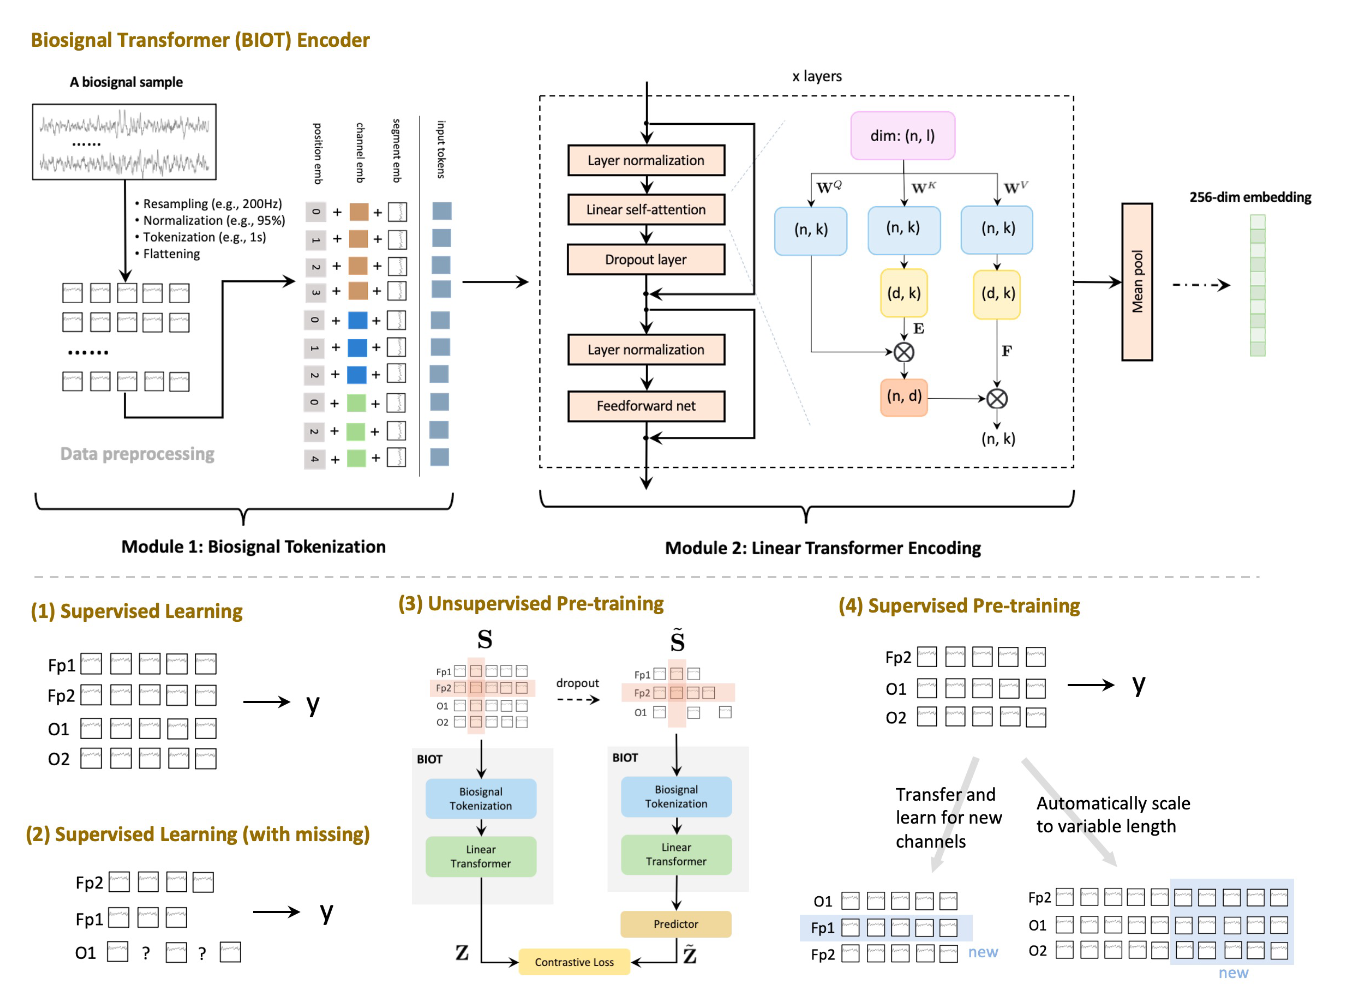
\includegraphics[width=\textwidth]{biot.png}
		\caption{معماری شبکه \english{BioT}}
		\label{biot}
		
	\end{figure}
	
	سپس تعامل بین این جملات با استفاده از ماژول ترنسفورمر خطی (نیم‌تصویر پایین) یاد گرفته می‌شوند. این مدل به صورت با نظارت می‌تواند داده‌های مختلف کامل و ناقص را برای پیش‌آموزش و \english{fine-tuning} بپیذیرد.
	
	\subsection{ساختار مدل}
	مدل از دو بخش انکودر و سر کلاسیفیکیشن\footnote{\english{Classification Head}} تشکیل شده‌است.\\
	
	سر کلاسیفیکیشن از یک تابع فعالساز \english{ELU}\footnote{\english{Exponential Linear Unit}} و یک لایه خطی تشکیل شده‌است که با تبدیل $xA^T + b$ انکودینگ ساخته شده را به یک وکتور با اندازه تعداد کلاس‌ها می‌برد که بیانگر احتمال این است که آن ورودی در هر کدام از آن کلاس‌ها باشد.\\
	
	بخش انکودر نیز ابتدا یک امبدینگ اولیه ساخته و سپس آن را به ترانسفورمر داده تا برای پنجره مورد نظر یک امبدینگ نهایی بسازد. در قسمت پیش‌رو به تفصیل این دو بخش توضیح داده شده‌اند.
	\subsubsection{امبدینگ اولیه}
	\subsubsection{بخش ترانسفورمر}
	بخش انکودر نیز ابتدا یک امبدینگ از ورودی ساخته و سپس آن را به یک ترانسفورمر با توجه خطی\footnote{\english{Linear Attention Transformer}} پاس می‌دهد. سپس خروجی ترانسفورمر که یک تنسور به ابعاد
	$(batch_size, combined_seq_len, emb_size)$
	است را با میانگین‌گیری در بعد اول تبدیل به تنسوری به ابعاد
	 $(batch_size, emb_size)$
	 می‌کنیم، تا برای هر پنجره از هر سیگنال‌ها به یک امبدینگ برسیم که برگرفته از اطلاعات کل پنحره در طول زمان است.\\
	 
	
	\subsection{مراحل خوراندن داده به مدل}
	برای آماده‌سازی داده خام و خوراندن آن به مدل \english{BioT} می‌بایست چندین کار انجام داد.\\
	
	پس از تمیزسازی دادگان که در بالا گفته شد، برای هر سوژه یک فایل \english{pickle} ساخته می‌شود که مجموع 15 فایل می‌شود. هر یک از این فایل‌ها یک دیکشنری به فرمت شکل \ref{fig:struct2} است، که هر یک از آنها یک تنسور است. طول تنسور تک بعدی \english{label} 4 برابر ثانیه‌های آن سوژه و ابعاد باقی تنسورهای سیگنال‌ها برابر
	
	$(\text{4برابر ثانیه‌ها}, \text{تعداد کانال‌ها}, \text{فرکانس سیگنال})$
	
	است.\\
	علت 4 برابر شدن ثانیه‌ها استفاده از ربع ثانیه به عنوان واحد زمانی است.  همچنین تعداد کانال‌ها برای همه به جز \english{ACC} برابر 1 است.\\
	
	
	\subparagraph{تغییر فرکانس}
	
	فرکانس مناسب برای مدل \english{BioT} برابر 200 هرتز است. بنابرین برای هر یک از سیگنال‌ها فرکانس سیگنال را به 200 تبدیل می‌کنیم. همچنین در کانال‌های مختلف میانگین می‌گیریم (در حقیقت این کار به جز بر \english{ACC} بر سیگنال دیگری تاثیری ندارد). در نهایت ابعاد هر یک از سیگنال‌ها به شکل 
	
	$(\text{4برابر ثانیه‌ها}, \text{200})$
	
	در می‌آید.\\
	
	برای تغییر فرکانس از تابع \english{resample} از پکیج \english{scipy} بهره بردیم. این تابع از متود فوریه برای تبدیل فرکانس یک سیگنال استفاده می‌گند.
	
	\subparagraph{نرمال‌سازی}
	
	با توجه به خود مدل \english{BioT}، نرمال‌سازی به این صورت انجام می‌شود که سیگنال‌ها بر چندک 95-صدم تقسیم می‌شود.
	
	\subparagraph{تقسیم دادگان}
	
	همانند تمامی مقالات و کارهای انجام شده بر روی این دادگان، ما هم از روش  \english{LOSO} استفاده می‌کنیم. بدین ترتیب به ازای هر یک از سوژه‌‌ها،‌ آن را به عنوان تست و از 14 تای باقی‌مانده،‌ 10 تا را به عنوان داده آموزشی و 4 تای باقی‌مانده را به عنوان داده \english{validation} استفاده می‌کنیم.
	
	\subsection{استخراج ویژگی‌ها}
	برای تبدیل داده به فرم مناسب برای آموزش مدل‌های ماشین لرنینگ، یکی از روش‌های پرکاربرد و محبوب، استخراج ویژگی از پنجره‌های سری زمانی است. در کارهای مختلف از پنجره‌های با طول‌های متفاوت استفاده می‌کنند. برای مثال در \cite{art2020} از پنجره‌هایی به طول 1 ثانیه، 10 ثانیه\cite{art2021}، و حتی 30 ثانیه\cite{behnam2021} استفاده کردند. در مورد آخر، یکی از علل طول زیاد پنجره به دلیل استفاده از مدل \english{transformer} و بهره‌گیری از زمینه\footnote{\english{context}} است.\\
	
	
	
	\section{نتایج}
	\subsection{2 کلاسه}
	برای مقایسه آن با هر یک از کارها، این مدل را با استفاده از سیگنال‌ها و پنجره‌های هر یک از کارها مقایسه می‌کنیم.\\
	در ابتدا مقایسه را 2کلاسه (استرس و غیر استرس) انجام می‌دهیم. در جدول \ref{compare1} نتایج با دو روش اول که پنجره‌های یکسانی داشتند مقایسه شدند. میانگین \english{f1-score} برابر 91 درصد شد که دقتی نسبتا خوب محسوب می‌شود.  به دلیل محدودیت‌های محاسباتی به جای قدم‌های ربع ثانیه‌ای از قدم‌های 6 ثانیه‌ای استفاده شد که اینگونه تعداد داده‌های آموزش به نسبت کار \cite{transformer1} که بهترین کار بوده، بسیار کمتر (حدودا 25 برابر) بوده ولی با این حال دقت تنها 2 درصد کمتر بوده که با کاهش اندازه قدم‌ها این درصد نیز بهتر خواهد شد.
	
	\begin{table}[h]
		\begin{tabular}{|c|c|c|}
			
			\hline
			سوژه & امتیاز \english{F-1} & \english{Accuracy}\\
			\hline
			2&$0.78$&$0.70$\\
			3&$0.82$&$0.79$\\
			4&$0.90$&$0.88$\\
			5&$0.96$&$0.96$\\
			6&$0.90$&$0.89$\\
			7&$0.82$&$0.80$\\
			8&$0.84$&$0.80$\\
			9&$0.80$&$0.73$\\
			10&$0.96$&$0.96$\\
			11&$0.90$&$0.90$\\
			13&$0.96$&$0.96$\\
			14&$0.70$&$0.73$\\
			15&$0.96$&$0.96$\\
			16&$0.98$&$0.98$\\
			17&$0.70$&$0.72$\\
			\hline
			مجموع&$0.91$&$0.93$\\
			\hline
		\end{tabular}
		\caption{نتایج \english{BioT} با پنجره 60 ثانیه و قدم‌های ربع ثانیه‌ای. سیگنال های \english{BVP}، \english{EDA} و دمای مج استفاده شدند.}
		\label{compare1}
		
	\end{table}
	
	
	\subsection{3 کلاسه}
	با بهره‌گیری از این مدل قدرتمند به نتایج بسیار بهتری در کلاس‌بندی با 3 کلاس خواهیم رسید. 3 کلاس عبارتند از استرس،‌ خوشحالی و عادی.\\
	
	\begin{table}[h]
		\begin{tabular}{|c|c|c|}
			\hline
			سوژه & امتیاز \english{F-1} & \english{Accuracy}\\
			\hline
			2&0.92&0.91\\
			3&0.78&0.73\\
			4&0.96&0.96\\
			5&0.98&0.98\\
			6&0.84&0.80\\
			7&0.84&0.83\\
			8&0.86&0.83\\
			9&0.80&0.73\\
			10&0.87&0.87\\
			11&0.73&0.75\\
			13&0.96&0.96\\
			14&0.57&0.59\\
			15&0.96&0.96\\
			16&1.00&1.0\\
			17&0.70&0.72\\
			\hline
			مجموع&0.91&0.90\\
			\hline
		\end{tabular}
		\caption{همانند \ref{compare1}، با تفاوت اینکه در اینجا 3 کلاس را مقایسه کردیم.}
		\label{compare2}
		
	\end{table}
	
	
	در جدول \ref{compare2} نتایج برای 3 کلاس با تنظیمات مشابه \ref{compare1} آورده شده‌است. امتیاز \english{f-1} به طور فوق‌العاده‌ای به بیش از 90\% رسید که بسیار بهتر از امتیازهای 3 کلاسه دیگر مقالات است!\\
	
	\begin{figure}[h]
		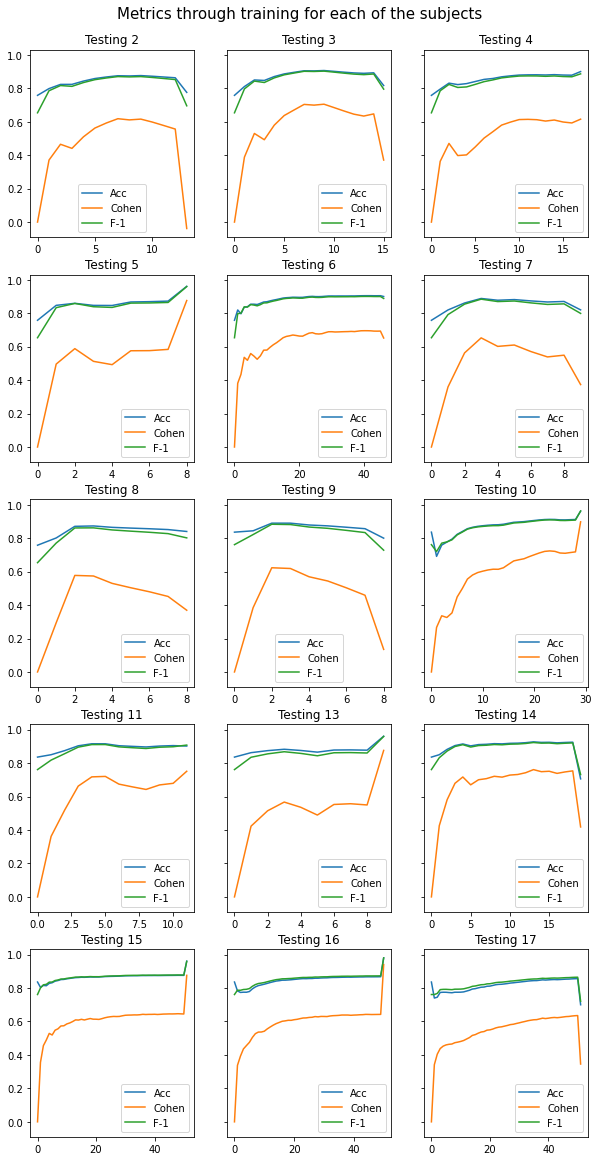
\includegraphics[width=0.6\textwidth]{traj1.png}
		\caption{روند پیشرفت دقت و معیارهای دیگر در طول فرایند یادگیری. نقطه آخر این نمودارها بیانگر دقت بر روی تست است.}
		\label{traj1}
	\end{figure}
	
	در شکل \ref{traj1} دقت، امتیاز \english{Cohen} و \english{F-1} در طول روند یادگیری برای 3 کلاس می‌باشد. حد بالای تعداد \english{epoch} ها برابر 50 بوده، ولی همانطور که مشاهده می‌کنیم، 12 تا از آنها قبل از این مقدار همگرا شدند و به 50 نرسیدند که 10 تای آنها به زیر 20 \english{epoch} برای همگرایی نیاز داشتند.\\
	
	نقطه آخر هر یک از نمودارها، آن معیار برای داده تست می‌باشد و دلیل جهش ناگهانی در آخر نمودارها همین نکته است. از بین این 15تا تنها در 6 سوژه برای داده تست افت بدی را در معیارها شاهد بودیم که بیانگر انطباق بیش‌ازحد\footnote{\english{Over fit}} می‌باشد.\\
	 
	\newpage
	\begin{thebibliography}{9}
		\bibitem{wesad}
		\href{https://eclass.hmu.gr/modules/document/file.php/ECE224/Project/2018_Introducing%20WESAD%2C%20a%20Multimodal%20Dataset%20for%20Wearable%20Stress%20and%20Affect%20Detection.pdf}{\english{Schmidt, P., Reiss, A., Duerichen, R., Marberger, C., and Van Laerhoven,
			K. (2018, October). Introducing wesad, a multimodal dataset for wearable
			stress and affect detection. In Proceedings of the 20th ACM international
			conference on multimodal interaction (pp. 400-408)}}
		
		\bibitem{empatica}
		\href{https://dl.acm.org/doi/pdf/10.1145/3568231.3568242}{\english{Fauzi, M. A., Yang, B., and Yeng, P. (2022, November). Improving Stress Detection Using Weighted Score-Level Fusion of Multiple Sensor. In Pro-ceedings of the 7th International Conference on Sustainable Information Engineering and Technology (pp. 65-71).}}
		
		\bibitem{respiban}
		\href{https://ieeexplore.ieee.org/stamp/stamp.jsp?arnumber=9437232}{\english{Iqbal, T., Redon-Lurbe, P., Simpkin, A. J., Elahi, A., Ganly, S., Wijns, W.,
			and Shahzad, A. (2021). A sensitivity analysis of biophysiological responses
			of stress for wearable sensors in connected health. IEEE Access, 9, 93567-
			93579}}
		
		\bibitem{art2020}
		\href{https://www.researchgate.net/profile/Pramod-Bobade/publication/344052913_Stress_Detection_with_Machine_Learning_and_Deep_Learning_using_Multimodal_Physiological_Data/links/5fce329da6fdcc697be8c5a8/Stress-Detection-with-Machine-Learning-and-Deep-Learning-using-Multimodal-Physiological-Data.pdf}{\english{Bobade, P., and Vani, M. (2020, July). Stress detection with machine learning and deep learning using multimodal physiological data. In 2020 Second International Conference on Inventive Research in Computing Applications (ICIRCA) (pp. 51-57). IEEE.}}
		
		\bibitem{art2021}
		\href{https://shoya.io/preprint/garg2021stress.pdf}{\english{Garg, P., Santhosh, J., Dengel, A., and Ishimaru, S. (2021, April). Stress detection by machine learning and wearable sensors. In 26th International Conference on Intelligent User Interfaces-Companion (pp. 43-45).}}
		
		\bibitem{behnam2021}
		\href{https://arxiv.org/pdf/2108.09737.pdf}{\english{Behinaein, B., Bhatti, A., Rodenburg, D., Hungler, P., and Etemad, A. (2021, September). A transformer architecture for stress detection from ecg. In Proceedings of the 2021 ACM International Symposium on Wearable Computers (pp. 132-134).}}
		
		\bibitem{transformer1}
		\href{https://arxiv.org/pdf/2303.17611}{\english{Wu, Y., Daoudi, M., \& Amad, A. (2023). Transformer-based self-supervised multimodal representation learning for wearable emotion recognition. IEEE Transactions on Affective Computing, 15(1), 157-172.}}
		
		\bibitem{convAE1}
		\href{https://ieeexplore.ieee.org/abstract/document/9871958/}{\english{Rovinska, S., \& Khan, N. (2022, July). Affective State Recognition with Convolutional Autoencoders. In 2022 44th Annual International Conference of the IEEE Engineering in Medicine \& Biology Society (EMBC) (pp. 4664-4667). IEEE.}}
	\end{thebibliography}
	
\end{document}